
\documentclass[calculator,steamtables,datasheet,solutions]{exam_newMarcus2}
%\documentclass[calculator,allquestions,datasheet]{exam_newMarcus2}

% The full list of class options are
% calculator : Allows approved calculator use.
% datasheet : Adds a note that data sheet are attached to the exam.
% handbook : Allows the use of the engineering handbook.
% resit : Adds the resit markings to the paper.
% sample : Adds conspicuous SAMPLE markings to the paper
% solutions : Uses the contents of \solution commands (and \solmarks) to generate a solution file

\usepackage{pdfpages} 
\usepackage{lscape,comment}
 
\coursecode{EX3029}%%
\coursetitle{Chemical Thermodynamics}

\examtime{09.00--12.00}%
\examdate{14}{12}{2015}% 
\examformat{Candidates must attempt \textit{all} questions, each of which carries equal (20) marks.  All thermodynamic symbols have their usual meanings unless otherwise stated.}

\newcommand{\frc}{\displaystyle\frac}
\newcommand{\br}[1]{\!\left( #1 \right)}
\newcommand{\abs}[1]{\left| #1 \right|}
\newcommand{\fracd}[2]{\frac{\mathrm{d} #1}{\mathrm{d} #2}}
\newcommand{\fracp}[2]{\frac{\partial #1}{\partial #2}}
\renewcommand{\d}[1]{\mathrm{d} #1 } 
\newcommand{\Ma}{\mathrm{M\!a}} 



\begin{document}

%%%
%%% Question 01
%%%
\begin{question}
%
\begin{enumerate}[(a)]
%%% Johannes T3Q4
\item Assuming $S = S\left(P,V\right)$ and taking into consideration that,
\begin{displaymath}
\left(\frc{\partial S}{\partial T}\right)_{V} = \frc{C_{V}}{T}\;\;\;\text{ and }\;\;\; \left(\frc{\partial S}{\partial T}\right)_{P} = \frc{C_{P}}{T}
\end{displaymath}
Prove that 
\begin{displaymath}
\d S = \frc{C_{V}}{T}\left(\frc{\partial T}{\partial P}\right)_{V}\d P + \frc{C_{P}}{T}\left(\frc{\partial T}{\partial V}\right)_{P}\d V
\end{displaymath}~\marks{8}
%
\solution{As entropy is expressed as a function of pressure and molar volume, we can write it in differenctial form as,~\solmarks{2/8}
\begin{displaymath}
  dS = \left(\frc{\partial S}{\partial P}\right)_{V}dP + \left(\frc{\partial S}{\partial V}\right)_{p}dV 
\end{displaymath}
We can rewrite this equation as~\solmarks{3/8}
\begin{displaymath}
dS = \left(\frc{\partial S}{\partial T}\right)_{V}\left(\frc{\partial T}{\partial P}\right)_{V}dP + \left(\frc{\partial S}{\partial T}\right)_{p}\left(\frc{\partial T}{\partial V}\right)_{p}dV
\end{displaymath}
As $\left(\frc{\partial S}{\partial T}\right)_{V}=\frc{C_{v}}{T}$ and $\left(\frc{\partial S}{\partial T}\right)_{P}=\frc{C_{P}}{T}$, ~\solmarks{3/8}
\begin{displaymath}
dS = \frc{C_{v}}{T}\left(\frc{\partial T}{\partial P}\right)_{V}dP + \frc{C_{P}}{T}\left(\frc{\partial T}{\partial V}\right)_{p}dV
\end{displaymath}
}

%%%
%%% Johannes Lecture Example
%%%
\item\label{LectExample} The liquid phase esterification of acetic acid with ethanol is given by,
\begin{displaymath}
CH_{3}COOH + C_{2}H_{5}OH  \Longleftrightarrow  CH_{3}COOC_{2}H_{5} + H_{2}O.
\end{displaymath}
Calculate the equilibrium mole fraction of ethyl acetate at 100$^{\circ}$C, given that initially there were 1 mole of acetic acid and 1 mole of ethanol. The standard enthalpy and Gibbs free energy of the reaction at 25$^{\circ}$C are -3.64 kJ.mol$^{-1}$ and -4.65 kJ.mol$^{-1}$, respectively. The van't Hoff equation is given by~\marks{12}
\begin{displaymath}
\frc{d}{dT}\left(\ln{K}\right) = - \frc{\Delta H_{298}^{o}}{RT^{2}}.
\end{displaymath}

%==========================
\solution{ Initially we have 1 mol of acetic acid (HAc) and 1 mol of ethanol (EtOH). We can calculate the mole fractions for all species as a function of the reaction coordinate, $\epsilon$~\solmarks{4/12}
\begin{eqnarray}
 x_{\text{EtAc}} &=& \frc{\epsilon}{2+0.\epsilon} = \frc{\epsilon}{2} = x_{H_{2}O}  \nonumber \\
 x_{\text{HAc}} &=& \frc{1-\epsilon}{2} = x_{\text{EtOH}} \nonumber
\end{eqnarray}
Assuming ideal solution,~\solmarks{2/12}
\begin{displaymath}
  \prod\limits_{i=1}^{c=4} x_{i}^{\nu} = K = x_{\text{HAc}}^{-1}\;x_{\text{EtOH}}^{-1}\;x_{\text{EtAc}}\;x_{H_{2}O} \Longrightarrow K = \frc{\epsilon^{2}}{\left(1-\epsilon\right)^{2}}
\end{displaymath} 
Thus, by calculating $K$, we can obtain $\epsilon$ and then $x_{\text{EtAc}}$. $K$ (temperature-dependent) can be obtained from the Gibbs free energy,~\solmarks{2/12}
\begin{displaymath}
   \ln{K_{298}} = -\frc{\Delta G_{298}^{o}}{RT} = \frc{4650.0}{8.314\times 298.15} = 1.8759 \Longrightarrow K_{298} = 6.5267
\end{displaymath}
Now, in order to calculate $K$ at 373.15 K, we can integrate the van't Hoff equation from 298.15 K to 373.15 K~\solmarks{2/12}
\begin{eqnarray}
   && \int\limits_{K_{298}}^{K_{373}} d\left(\ln{K}\right) = - \int\limits_{298.15}^{373.15}\frc{\Delta H_{298}^{o}}{RT^{2}} dT \nonumber \\
   && \ln\left(\frc{K_{373}}{K_{298}}\right) = - \frc{-3640.0}{8.314}\left(\frc{1}{373.15}-\frc{1}{298.15}\right) \Longrightarrow K_{373} = 4.8586 \nonumber
\end{eqnarray}
Now we can calculate the reaction coordinate,
\begin{displaymath}
   K_{373} = \frc{\epsilon^{2}}{\left(1-\epsilon\right)^{2}} \Longrightarrow \epsilon= 0.6879
\end{displaymath} 
Thus ~\solmarks{2/12}  
\begin{displaymath}
x_{\text{EtAc}} = \frc{\epsilon}{2} = 0.3440
\end{displaymath}
%==========================
 }
%
\end{enumerate}
%
\end{question}
\clearpage


%%%
%%% Question 02
%%%
\begin{question}
\begin{enumerate}[(a)]
% LectureNotes_Nguyen (pg 89)
\item Show that the van der Waals equation of state (vdW EOS),
\begin{displaymath}
  P = \frc{RT}{V-b} - \frc{a}{V^{2}}
\end{displaymath} 
can be expressed as a cubic polynomial equation in $Z$ (compressibility coefficient),
\begin{displaymath}
Z^{3} -(1+B)Z^{2} +AZ -AB = 0 
\end{displaymath}
with $B=bP/(RT)$ and $A=aP/(RT)^{2}$.~\marks{7}

%==========================
\solution{We can rearrange the vdW EOS,~\solmarks{2/7}
\begin{displaymath}
   P = \frc{RT}{V-b} - \frc{a}{V^{2}} \Longrightarrow \frc{PV}{RT} = \frc{V}{V-b} - \frc{a}{RTV} = \frc{1}{1-\frc{b}{V}} - \frc{a}{RTV}
\end{displaymath}
Eliminating $V$ as $V=ZRT/P$,~\solmarks{1/7}
\begin{displaymath}
   Z = \left(1-\frc{bP}{ZRT}\right)^{-1} - \frc{aP}{Z\left(RT\right)^{2}} = \frc{ZRT}{ZRT-bP}-\frc{aP}{Z\left(RT\right)^{2}}
\end{displaymath}
Manipulating this expression,~\solmarks{3/7}
\begin{eqnarray}
   && Z^{2}R^{2}T^{2}\left(ZRT-bP\right) = Z^{2}\left(RT\right)^{3} - aP\left(ZRT-bP\right) \nonumber \\
   && Z^{3} - \frc{bP}{RT}Z^{2} - Z^{2} -\frc{aP}{\left(RT\right)^{2}}Z + ab\frc{P^{2}}{\left(RT\right)^{3}} = 0 \nonumber
\end{eqnarray}
with $B=bP/(RT)$, $A=aP/(RT)^{2}$ and $AB=ab\frc{P^{2}}{\left(RT\right)^{3}}$,~\solmarks{1/7}
\begin{displaymath}
Z^{3} -(1+B)Z^{2} +AZ -AB = 0 
\end{displaymath}
}
%==========================

\item Calculate the fugacity of gaseous CO$_{2}$ at 310 K and 1.4$\times$10$^{6}$ Pa using the van der Waals equation of state (EOS), with $a=$ 0.3658 Pa.m$^{6}$/mol$^{2}$, $b=$ 4.286$\times$10$^{-5}$ m$^{3}$/mol. Given,~\marks{13}
\begin{displaymath}
\ln{\left(\frc{f}{P}\right)} = -\ln{\left(1-\frc{b}{V}\right)} - \frc{a}{RTV} - \ln{Z} +\left(Z-1\right).
\end{displaymath}
Use the largest real root of the cubic polynomial in $Z$ to represent the gaseous phase.

%====================
\solution{Solving the cubic polynomial in $Z$, with $B=bP/(RT)$ and $A=aP/(RT)^{2}$,~\solmarks{5/13}
\begin{eqnarray}
Z^{3} -(1+B)Z^{2} +AZ -AB = 0 & \Longrightarrow& A = 7.7095\times 10^{-2}\; ;\; B = 2.3281\times 10^{-2} \nonumber \\ 
 &\Longrightarrow& Z = 0.9436 \nonumber
\end{eqnarray}
Now for the fugacity equation, either
\begin{eqnarray}
&& \ln{\left(\frc{f}{P}\right)} = -\ln{\left(1-\frc{b}{V}\right)} - \frc{a}{RTV} - \ln{Z} +\left(Z-1\right) \nonumber \\
&& \text{or} \nonumber \\
&&  \ln{\left(\frc{f}{P}\right)} = -\ln{\left(1-\frc{B}{Z}\right)} - \frc{A}{Z} - \ln{Z} +\left(Z-1\right) \nonumber
\end{eqnarray}
leads to $f =\; 1.32\times 10^{6}$ Pa.~\solmarks{8/13}

}
%====================
%
\end{enumerate}
%
\end{question}

\clearpage

%%%
%%% Question 03
%%%
\begin{question}
%
%%%
%%% Jeff Solved Example 3 ==> Sandler Example 10.1.4 (page 504)
%%%
 An ideal liquid mixture of 25 mol$\%$ n-pentane $\left(nC_{5}\right)$, 45 mol$\%$ n-hexane $\left(nC_{6}\right)$ and 30 mol$\%$ n-heptane $\left(nC_{7}\right)$, initially at 69$^{\circ}$C and high pressure, is partially vaporised by isothermically lowering the pressure to 1.013 bar. Calculate the relative amounts of vapour and liquid in equilibrium and their compositions.~\marks{20}
%======================
\solution{ From the Antoine equation, we can calculate the saturation pressure of the species $P_{\text{C}_{5}}^{sat}=$ 2.721 bar, $P_{\text{C}_{6}}^{sat}=$ 1.024 bar, $P_{\text{C}_{7}}^{sat}=$ 0.389 bar.~\solmarks{3/20} Assuming ideal solution,
\begin{displaymath}
\frc{y_{i}}{x_{i}} = K_{i} = \frc{P_{i}^{sat}}{P}
\end{displaymath}
Thus $K_{\text{C}_{5}}=$ 2.6861, $K_{\text{C}_{6}}=$ 1.0109 and $K_{\text{C}_{7}}=$ 0.3840~\solmarks{3/20}, therefore~\solmarks{2/20}
\begin{eqnarray}
&& y_{\text{C}_{5}} = x_{\text{C}_{5}}K_{\text{C}_{5}},\;\; y_{\text{C}_{6}} = x_{\text{C}_{6}}K_{\text{C}_{6}},\;\; y_{\text{C}_{7}} = x_{\text{C}_{7}}K_{\text{C}_{7}} \nonumber \\
&& \sum\limits_{i=1}^{3}x_{i} = x_{\text{C}_{5}} + x_{\text{C}_{6}} + x_{\text{C}_{7}} = 1  \nonumber \\
&& \sum\limits_{i=1}^{3}y_{i} = y_{\text{C}_{5}} + y_{\text{C}_{6}} + y_{\text{C}_{7}} = 1  = K_{\text{C}_{5}}x_{\text{C}_{5}} + K_{\text{C}_{6}}x_{\text{C}_{6}} + K_{\text{C}_{7}}x_{\text{C}_{7}} \nonumber
\end{eqnarray}
The mass balance is,~\solmarks{1/20}
\begin{eqnarray}
&& L + V = 1 \nonumber \\
&& x_{i}L + y_{i}V = z_{i} \nonumber 
\end{eqnarray}
with $z_{i}=\left(0.25\;\;0.45\;\;0.30\right)^{T}$. Rearranging this set of equations lead to a non-linear expression in $L$,~\solmarks{3/20}
\begin{displaymath}
\frc{0.25}{\left(1-K_{\text{C}_{5}}\right)L+K_{\text{C}_{5}}} + \frc{0.45}{\left(1-K_{\text{C}_{6}}\right)L+K_{\text{C}_{6}}} +  \frc{0.30}{\left(1-K_{\text{C}_{7}}\right)L+K_{\text{C}_{7}}} = 1 
\end{displaymath}
Solving this equation leads to $L=0.5748$ and $V=0.4252$~\solmarks{2/20}. Calculating the molar fractions of the species:~\solmarks{6/20}
\begin{center}
\begin{tabular}{c c c c}
\hline
                 & {\bf n-C$_{5}$} &  {\bf n-C$_{6}$} &  {\bf n-C$_{7}$} \\
\hline
  {\bf x$_{i}$}   & 0.1456         &  0.4479         & 0.4065    \\
  {\bf y$_{i}$}   &  0.3911        &  0.4528         & 0.1561    \\
\hline
\end{tabular} 
\end{center}

}
%======================

For this problem, use 
\begin{displaymath}
   \ln P_{i}^{\text{sat}} = A_{i} - \frc{B_{i}}{RT}
\end{displaymath} 
with [P] = bar, [T] = K and $\left[\text{B}_{i}\right]$ = J.mol$^{-1}$ and
    \begin{center}
       \begin{tabular}{l l l} 
          $A_{nC_{5}}=10.422$ & $A_{nC_{6}}=10.456$ & $A_{nC_{7}}=11.431$ \\
          $B_{nC_{5}}=26799$  & $B_{nC_{6}}=29676$  & $B_{nC_{7}}=35200$  
       \end{tabular}
    \end{center}
%
\end{question}

\clearpage

%%%
%%% Question 04
%%%
\begin{question}
%
\begin{enumerate}[(a)]

%%%
%%% Johannes Problem 2 (Tutorial 5)
%%%
\item\label{Tut05P2} A process stream contains light species 1 and heavy species 2. A relatively pure liquid stream containing mostly 2 is obtained through a single-stage liquid/vapour separator. Equilibrium mole fractions are $x_{1}$ = 0.002 and $y_{1}$ = 0.950. Assuming that the modified Raoult's law applies, 
\begin{displaymath}
  y_{i} P = x_{i}\gamma_{i}P_{i}^{\text{sat}},
\end{displaymath} 
determine $T$ and $P$ for the separator. The activity coefficients for the liquid phase are given by,
\begin{displaymath}
\ln\gamma_{1} = 0.93x_{2}^{2} \;\;\;\;\;\text{ and }\;\;\;\;\;\ln\gamma_{2}=0.93x_{1}^{2},
\end{displaymath}
and the saturated vapour pressure is given by,
\begin{displaymath}
\ln P^{\text{sat}} = A - \frc{B}{T}\;\;\;\text{with [P] = bar and [T] = [B] = K},
\end{displaymath} 
with $A_{1}=$ 10.08, $B_{1}=$ 2572.0, $A_{2}=$  11.63 and $B_{2}=$ 6254.0.~\marks{13}

%===================
\solution{Given,
\begin{eqnarray}
&& x_{1} = 0.002 \;\;\Longrightarrow \;\; x_{2} = 0.998 \nonumber \\
&& y_{1} = 0.950 \;\;\Longrightarrow \;\; y_{2} = 0.050 \nonumber
\end{eqnarray}
Calculating the activity coefficient,~\solmarks{2/13},
\begin{eqnarray}
&& \ln{\gamma_{1}} = 0.93 x_{2}^{2} \;\;\Longrightarrow \;\; \gamma_{1} = 2.5251 \nonumber \\
&& \ln{\gamma_{2}} = 0.93 x_{1}^{2} \;\;\Longrightarrow \;\; \gamma_{2} = 1.0000 \nonumber
\end{eqnarray}
The modified Raoult's law,~\solmarks{4/13}
\begin{eqnarray}
&& y_{i}P=x_{i}\gamma_{1}P_{i}^{sat} \;\; \Longrightarrow \;\; P=\frc{x_{i}\gamma_{i}P_{i}^{sat}}{y_{i}} \nonumber \\
&& \frc{P_{1}^{sat}}{P_{2}^{sat}} = \frc{x_{2}\gamma_{2}y_{1}}{x_{1}\gamma_{1}y_{2}} = 3754.7028 = \frc{\exp{\left(A_{1}-\frc{B_{1}}{T}\right)}}{\exp{\left(A_{2}-\frc{B_{2}}{T}\right)}}\nonumber
\end{eqnarray}
Solving this equation results in $T=376.45$ K~\solmarks{3/13}. The pressure can now be obtained,~\solmarks{4/13}
\begin{displaymath}
  P=\frc{x_{i}\gamma_{1}P_{1}^{sat}}{y_{1}} = 0.1368\text{ bar}
\end{displaymath}
}
%==================

% Nguyen (page 106, Ex 5.1-1)
\item Determine the temperature and composition of the first bubble created from a saturated liquid mixture of benzene and toluene containing 45 mol$\%$ percent of benzene at 200 kPa. Benzene and toluene mixtures may be considered as ideal. Given,~\marks{7}
\begin{displaymath}
\ln{P^{sat}} = A - \frc{B}{T+C}\;\;\text{ with [P] = kPa and  [T] = [B] = [C] = K},
\end{displaymath}
and
\begin{center}
\begin{tabular}{ c  c  c  c }
\hline
           & ${\bf A}$  &  ${\bf B}$  & ${\bf C}$ \\
\hline
Benzene    & 14.1603    &  2948.78    & -44.5633 \\
Toluene    & 14.2514    &  3242.38    & -47.1806 \\
\hline
\end{tabular}
\end{center}

%=================
\solution{From Raoult's law, 
\begin{displaymath}
y_{i} = \frc{x_{i}P_{i}^{sat}}{P}
\end{displaymath}
with benzene (1) and toluene (2),~\solmarks{1/7}
\begin{displaymath}
P = x_{1}P_{1}^{sat} + x_{2}P_{2}^{sat}
\end{displaymath}
leading to the bubble point temperature of the mixture benzene-toluene~\solmarks{3/7}
\begin{displaymath}
P = x_{1}\exp{\left(A_{1}-\frc{B_{1}}{T+C_{1}}\right)} + x_{2}\exp{\left(A_{2}-\frc{B_{2}}{T+C_{2}}\right)} \;\Longrightarrow\; T= 391.73\text{ K}
\end{displaymath}
Calculating the saturation pressure and mole fraction of benzene in the vapour phase,~\solmarks{3/7}
\begin{eqnarray}
&& P_{1}^{sat} = \exp{\left(A_{1}-\frc{B_{1}}{T - C_{1}}\right)} = 289.01\text{ kPa} \nonumber \\
&& y_{1} = \frc{x_{1}P_{1}^{sat}}{P} = 0.6503 \;\text { and } y_{2}=1-y_{1} = 0.3497 \nonumber
\end{eqnarray}
}
%=================

\end{enumerate}

\end{question}



\clearpage

%%%
%%% Question 06
%%%
\begin{question}
%


%%%
%%% SM &VN 11.13 (Tutorial 6, prob 5)
%%%
 The molar volume $\left(\text{in cm}^{3}\text{.mol}^{-1}\right)$ of a binary liquid mixture at $T$ and $P$ is given by:
\begin{displaymath}
V = 120 x_{1} + 70 x_{2} + \left( 15x_{1} + 8x_{2}\right)x_{1}x_{2} 
\end{displaymath}
\begin{enumerate}[(a)]
\item\label{first} Find expressions for the partial molar volumes of species 1 and 2 at $T$ and $P$.~\marks{7}
%===================
\solution{ Eliminating $x_{2}=1-x_{1}$ in the molar volume expression,~\solmarks{1/7}
\begin{eqnarray}
V &=& 120 x_{1} + 70 x_{2} + \left( 15x_{1} + 8x_{2}\right)x_{1}x_{2} \nonumber \\
  &=& 70 + 58x_{1}-x_{1}^{2}-7x_{1}^{3} \nonumber
\end{eqnarray}
The Gibbs-Duhen equation at constant $T$ and $P$ can be expressed as,
\begin{displaymath}
\overline{M}_{1} = M + x_{2}\frc{dM}{dx_{1}} \;\text{ and }\; \overline{M}_{2} = M - x_{1}\frc{dM}{dx_{1}}
\end{displaymath}
and are used to obtain $\overline{V}_{1}$ and $\overline{V}_{2}$. However we first need to calculate~\solmarks{2/7}
\begin{displaymath}
\frc{dV}{dx_{1}} = 58 - 2x_{1} - 21x_{1}^{2}
\end{displaymath}
Thus~\solmarks{4/7}
\begin{eqnarray}
\overline{V}_{1} &=& 128 - 2x_{1} - 20x_{1}^{2} + 14x_{1}^{3} \nonumber \\
\overline{V}_{2} &=& 70  + x_{1}^{2} + 14x_{1}^{3} \nonumber 
\end{eqnarray}
}
%===================

\item Show that these expressions satisfy the Gibbs-Duhem equation, $\sum\limits_{i}x_{i}d\overline{M}_{i}=0$, where $M$ is an intensive thermodynamic property.~\marks{5}

%=========================
\solution{From this relation,~\solmarks{1/5}
\begin{displaymath}
   x_{1}d\overline{V}_{1} + x_{2}d\overline{V}_{2} = 0\;\Longrightarrow \; x_{1}\frc{d\overline{V}_{1}}{dx_{1}} + x_{2}\frc{d\overline{V}_{2}}{dx_{1}} = 0
\end{displaymath}
Differentiating $\overline{V}_{i}$ with repect to $x_{1}$,~\solmarks{2/5}
\begin{displaymath}
\frc{d\overline{V}_{1}}{dx_{1}} = -2-40x_{1}+42x_{1}^{2} \;\text{ and }\; \frc{d\overline{V}_{2}}{dx_{1}}= 2x_{1}+42x_{1}^{2}
\end{displaymath}
Now applying it into the original equation,~\solmarks{2/5}
\begin{eqnarray}
x_{1} \left(-2-40x_{1}+42x_{1}^{2}\right) &=& \left(1-x_{1}\right)\left(2x_{1}+42x_{1}^{2}\right) \nonumber \\
0&=&0
\end{eqnarray}
This demonstrates the validity of the Gibbs-Duhen equation.
}
%=========================

 \item Plot values of $V$, $\overline{V}_{1}$ and $\overline{V}_{2}$ calculated by the given equation for $V$ and by the equations developed in (a) {\it vs} $x_{1}$. Label points $\overline{V}_{1}^{\infty}$ and $\overline{V}_{2}^{\infty}$ and show their values.~\marks{8} 
%=============
\solution{The plot is~\solmarks{2/8}
\begin{center}
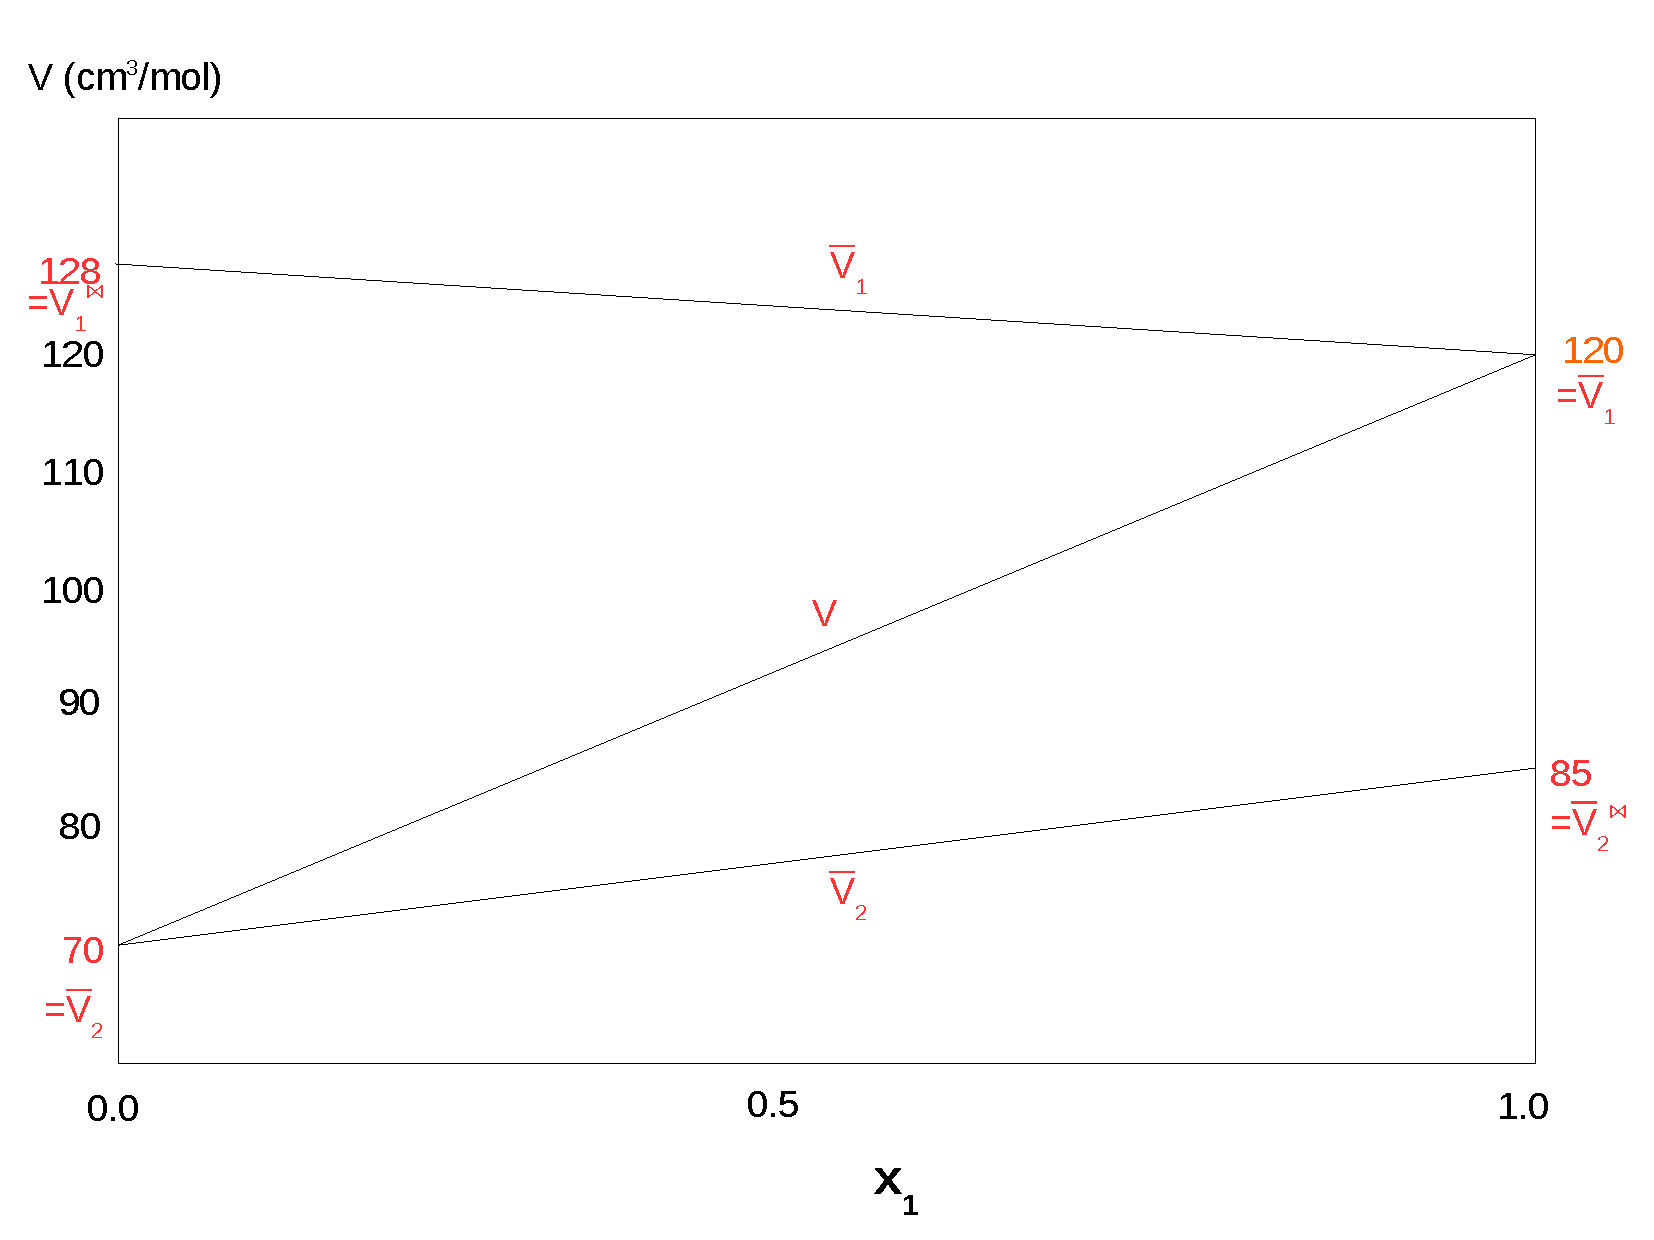
\includegraphics[width=15.cm,height=13.cm,clip]{./Pics/Vxplot}
\end{center}
where~\solmarks{6/8}
\begin{center}
\begin{tabular}{c c c}
\hline
              &  ${\bf x_{1}=0.0}$ & ${\bf x_{1}=1.0}$ \\
\hline
${\bf V}$     &     70            & 120              \\
${\bf \overline{V}_{1}}$ & 128   & 120               \\
${\bf \overline{V}_{2}}$ & 70   & 85               \\
\hline
\end{tabular}
\end{center}
}
%=============
\end{enumerate}
\end{question}

\vfill
\paperend

\clearpage

\begin{center}
\Large{List of Equations}
\end{center}

\begin{itemize}
%%%
\item Generic cubic equation of state:
\begin{eqnarray}
&& Z= 1 + \beta - q\beta \frc{Z - \beta} {\left(Z+\varepsilon\beta\right)\left(Z+\sigma\beta\right)}  \;\;\text{(vapour and vapour-like roots)}\nonumber\\
&& Z= 1 + \beta + \left(Z + \epsilon\beta\right)\left(Z+\sigma\beta\right)\left(\frc{1+\beta-Z}{q\beta}\right)  \;\;\text{(liquid and liquid-like roots)}\nonumber\\
&& \text{with }\; \beta=\Omega\frc{P_{r}}{T_{r}} \;\;\text{ and } \;\; q=\frc{\Psi\alpha\left(T_{r}\right)}{\Omega T_{r}}  \nonumber \\
&&\alpha_{\text{SRK}} = \left[ 1 + \left( 0.480 + 1.574 \omega - 0.176\omega^{2}\right)\left(1-\sqrt{T_{r}}\right)\right]^{2}  \nonumber \\
&&\alpha_{\text{PR}} = \left[ 1 + \left( 0.37464 + 1.54226 \omega - 0.26992\omega^{2}\right)\left(1-\sqrt{T_{r}}\right)\right]^{2} \nonumber
\end{eqnarray} 
    \begin{center}
       \begin{tabular}{| l | c c c c c| }
       \hline
          {\bf EOS}  & {\bf $\alpha$} & {\bf $\sigma$}  & {\bf $\varepsilon$} & {\bf $\Omega$} & {\bf $\Psi$ } \\
       \hline
            vdW      & 1              & 0               & 0                  & 1/8            & 27/64          \\
            RK       & T$_{r}^{-1/2}$  & 1                & 0                  & 0.08664       & 0.42748        \\
           SRK       &$\alpha_{\text{SRK}}$& 1            & 0                   & 0.08664       & 0.42748        \\
            PR       &$\alpha_{\text{PR}}$& 1+$\sqrt{2}$   & 1-$\sqrt{2}$        & 0.07780        & 0.45724  \\
       \hline
       \end{tabular}
    \end{center}

%%%
\item Newton-Raphson (root-finder) method: $X_{i} = X_{i-1} - \frc{\mathcal{F}\left(X_{i-1}\right)}{d\mathcal{F}/dX\left(X_{i-1}\right)}$

%%%
\item Fundamental thermodynamic equations:\\
\begin{tabular}{c c c c}
$dU = dQ + dW$;  & $dH = dU + d(PV)$; & $dA = dU -d(TS)$; & $dG=dH-d(TS)$ \\
$dU = TdS - PdV$;& $dH = TdS + VdP$;  & $dA = -SdT - PdV$;& $dG = -SdT + VdP$ \\ 
\end{tabular}\\
\begin{tabular} {c c}
$dH = C_{p}dT + \left[ V - T\left(\frc{\partial V}{\partial T}\right)_{P}\right]dP$; &  $dS=C_{p}\frc{dT}{T} - \left(\frc{\partial V}{\partial T}\right)_{P}dP$ \\
$dU = C_{v}dT + \left[T\left(\frc{\partial P}{\partial T}\right)_{V} - P\right]dV$;  & $dS = C_{v}\frc{dT}{T} - \left(\frc{\partial P}{\partial T}\right)_{V}dV$
\end{tabular}

%%% 
\item Polytropic Relations:\\
\begin{displaymath} 
\frc{T_{2}}{T_{1}} =\left(\frc{P_{2}}{P_{1}}\right)^{\frac{\gamma-1}{\gamma}} = \left(\frc{V_{1}}{V_{2}}\right)^{\gamma-1}\;\; ; 
TV^{\gamma-1} =\text{ const};\; TP^{\frac{1-\gamma}{\gamma}}=\text{ const};\; PV^{\gamma}=\text{ const} 
\end{displaymath}

%%%
\item Raoult's Law:\\
\begin{displaymath}
y_{i}P = x_{i}P_{i}^{\text{sat}}\;\;\;\text{ and } \;\;\; y_{i}P = x_{i}\gamma_{i}P_{i}^{\text{sat}}\;\;\;\text{ with } i=1,2,\cdots N
\end{displaymath}

%%%
\item Henry's Law:\\
\begin{displaymath}
x_{i}\mathcal{H}_{i} = y_{i}P\;\;\;\text{ with } i=1,2,\cdots N
\end{displaymath}

%%%
\item Antoine Equation:\\
\begin{displaymath}
\log_{10} P^{\star} = A-\frc{B}{T+C}\;\;\;\text{ with P}^{\star}\text{ in mm-Hg and T in }^{\circ}\text{C}
\end{displaymath}

%%%
\item Solutions:\\
\begin{displaymath}
M^{\text{E}} = M - \sum\limits_{i=1}^{N} x_{i}M_{i}; \; \overline{M}_{1}=M+x_{2}\frc{d M}{dx_{1}};\; \overline{M}_{2} = M - x_{1}\frc{d M}{dx_{1}}
\end{displaymath}

\end{itemize}


\vfill 



%\begin{comment}
{
%  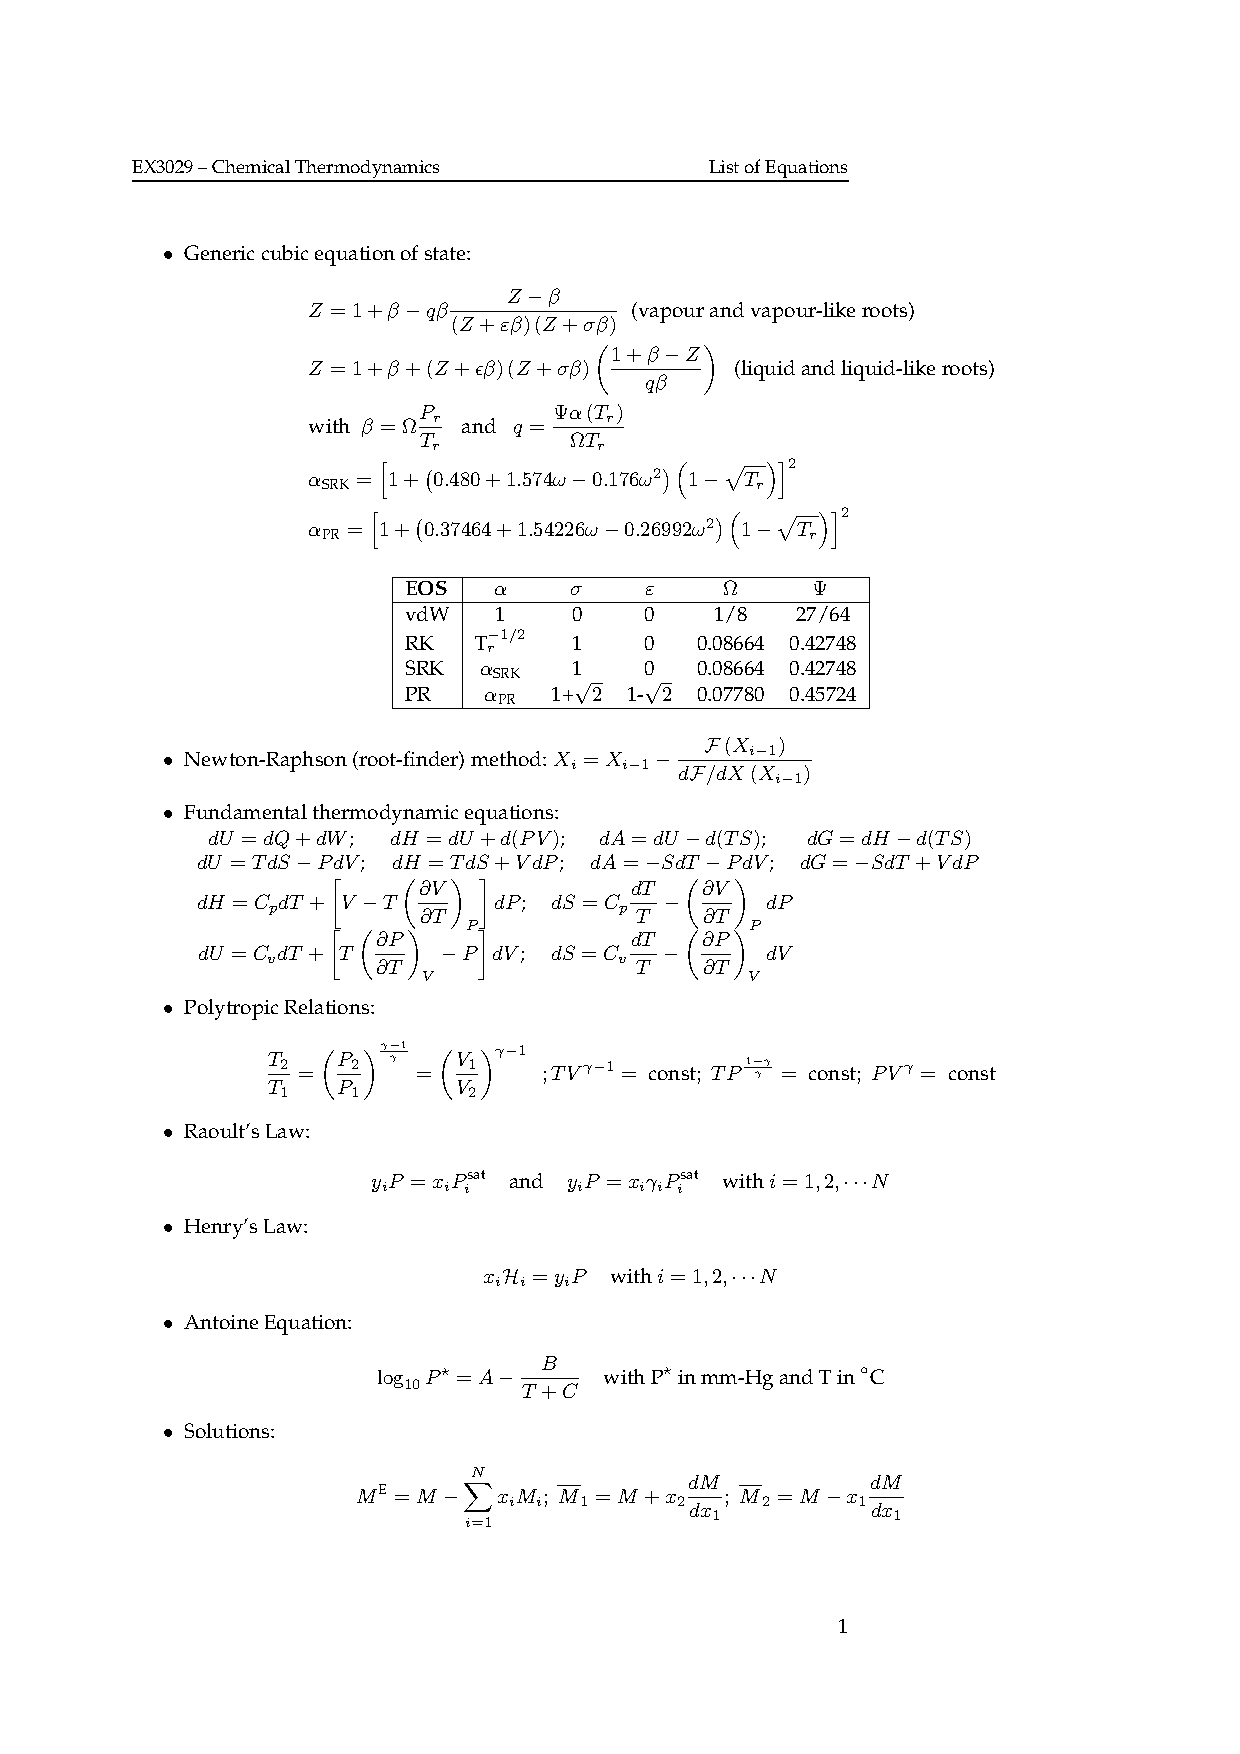
\includepdf[pages=-,fitpaper]{./Pics/EquationsList}
  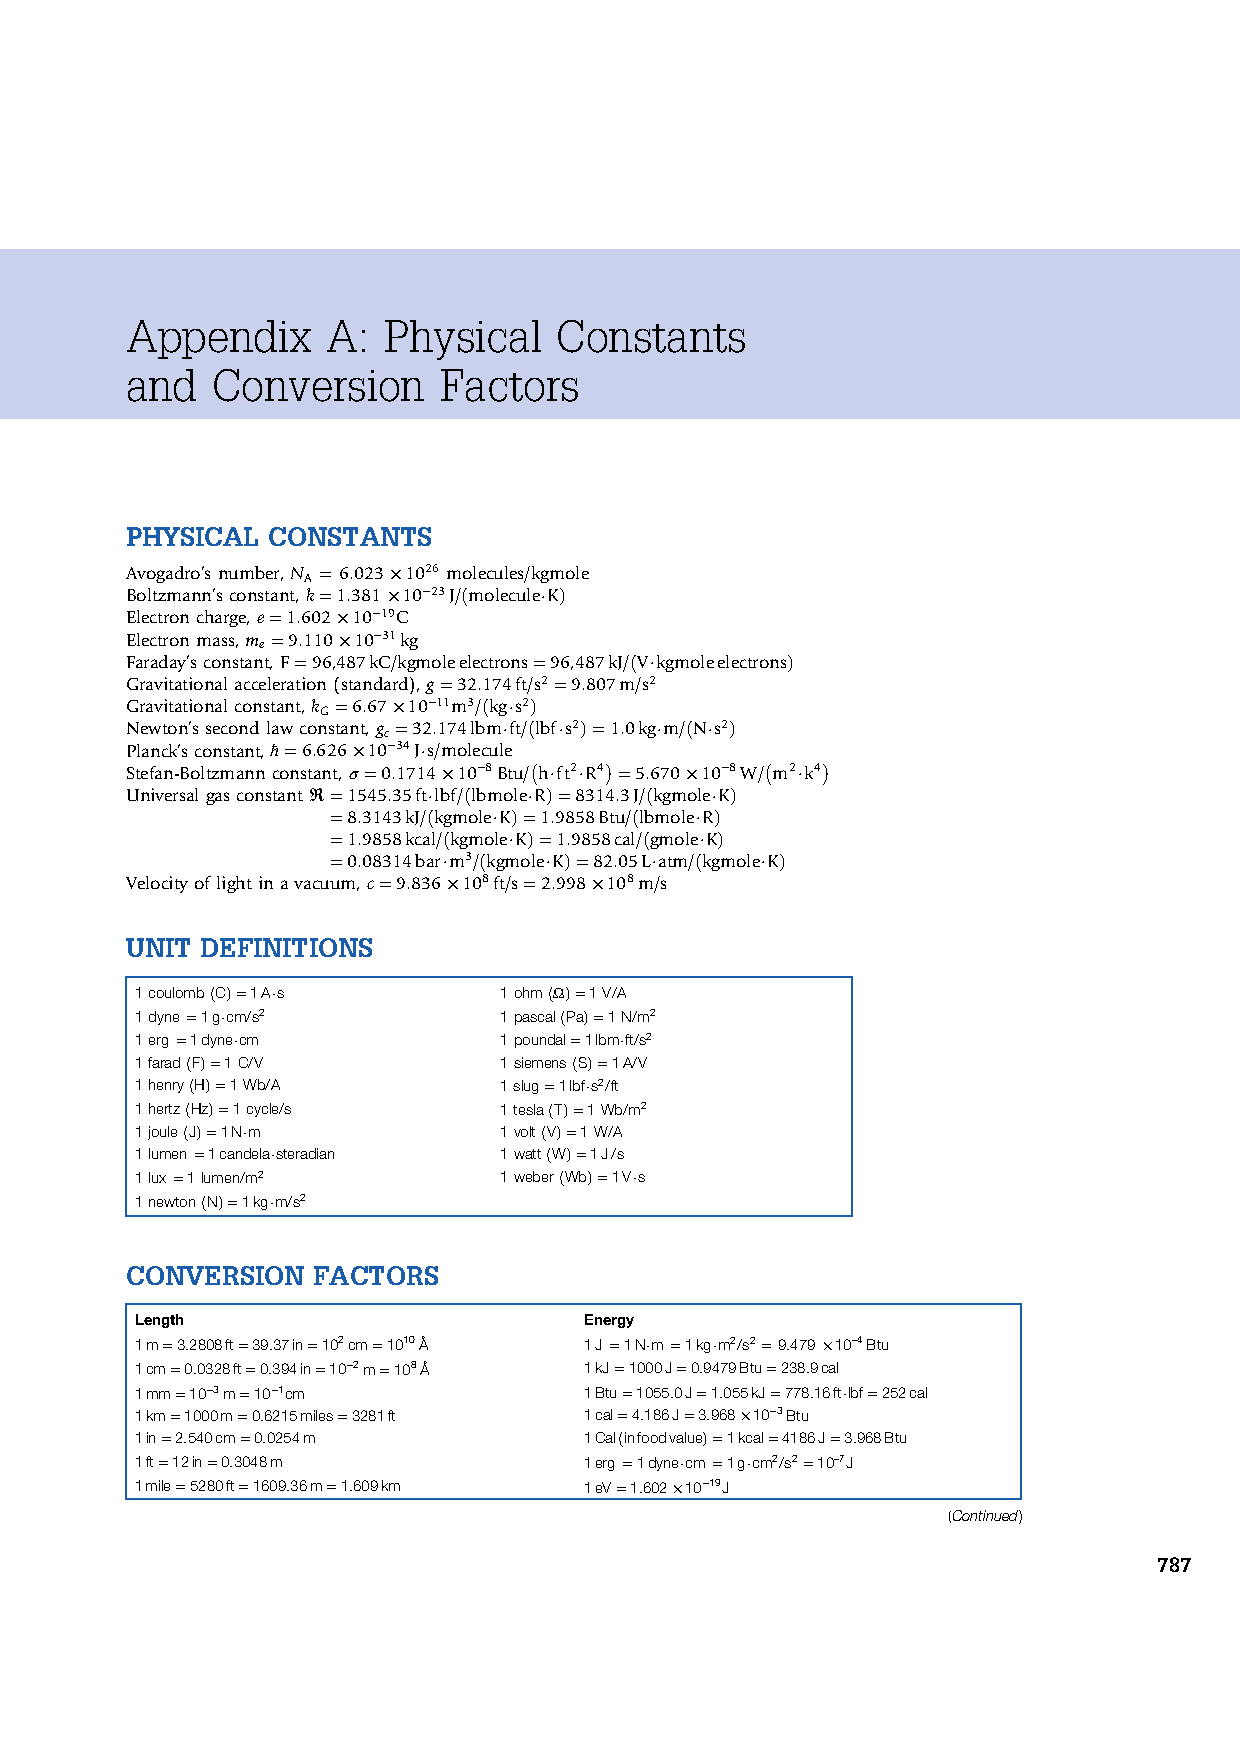
\includepdf[pages=-,fitpaper]{./Pics/ChemEng_UnitConv}
}
%\end{comment}



\end{document}
